\documentclass{article}
\usepackage{caption}
\usepackage{amssymb}
\usepackage{array}
\usepackage{geometry}
\usepackage{scrextend}
\usepackage{amsmath}
\usepackage{hyperref}
\usepackage{graphicx}
\usepackage{pdfpages}
\usepackage{multicol}
\usepackage{tabularx}
\usepackage{float}

\title{EE102 Homework 2}
\author{Jacob Guenther}

\geometry{
	a4paper,
	total={170mm,257mm},
	left=20mm,
	top=20mm,
}

\begin{document}

\includepdf[pages=1,pagecommand={}]{Lab_1_cover.pdf}

\section{Objective}
In this lab we review how to decode through hole resistors, how to measure resistance, and calculate the percent difference between values. We also apply the Steinhart-Hart equation (equation 2) to calculate the expected value of a thermistor. Further we gain experience plotting data.

\section{Equipment}
\begin{itemize}
	\item Agilent 34501A Multimeter
	\item Alligator Clips
	\item 680 $\Omega$ Resistor x4
	\item 1 k$\Omega$ Resistor
	\item 47 k$\Omega$ Resistor
	\item Digital Thermometer
	\item NTC-103 Thermistor
	\item Hot water
	\item Snow
\end{itemize}

\section{Setup}
For each resistor and the thermistor we use the following wiring diagram.

\begin{figure}[H]
	\begin{center}
		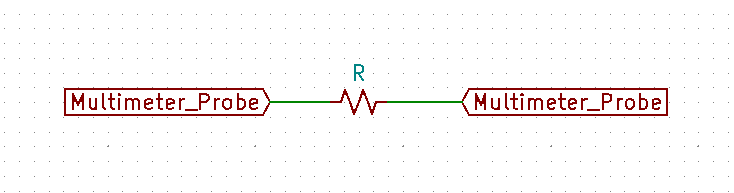
\includegraphics[width=8cm]{lab_1_figure_1}
	\end{center}
	\caption{On either side of the resistor is a one of the multimeter probes.}
\end{figure}

\section{Observations and Results}
\paragraph{}
As part of this lab we decode the color bands of the resistors provided using figure 2.

\begin{figure}[H]
	\begin{center}
		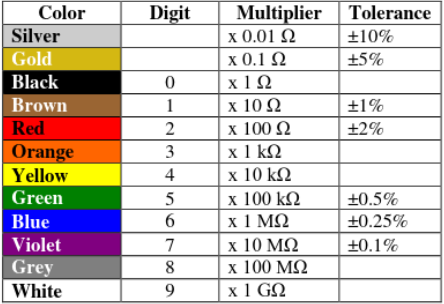
\includegraphics[width=8cm]{lab_1_figure_2}
	\end{center}
	\caption{Resistor color code}
\end{figure}

\paragraph{}
In table 1 we show or the decoded nominal values of the resistors, resistance measurements of the 680 $\Omega$ resistors, the 1 k$\Omega$ resistor, and the 47 k$\Omega$ resistor. Also in table 1 is the percent differences between the labeled value and measured value of each of the resistors calculated using equation 1.

\begin{table}[H]
\begin{tabularx}{\textwidth}{ | r | c | c | X | c | }
	\hline
	\textbf{Component} &
	\textbf{Component Marking} &
	\textbf{Decoded Value} &
	\textbf{Measured Resistance ($\Omega$)} &
	\textbf{\% Difference} \\
	\hline
	680 $\Omega$ Resistor & blu, gry, brn, gold & $68 \times 10^{1}=680 \Omega 5 \%$ & 672.17 & 1.151 \\
	\hline
	680 $\Omega$ Resistor & blu, gry, brn, gold & $68 \times 10^{1}=680 \Omega 5 \%$ & 671.9 & 1.191 \\
	\hline
	680 $\Omega$ Resistor & blu, gry, brn, gold & $68 \times 10^{1}=680 \Omega 5 \%$ & 678.33 & 0.246 \\
	\hline
	680 $\Omega$ Resistor & blu, gry, brn, gold & $68 \times 10^{1}=680 \Omega 5 \%$ & 675.31 & 0.69 \\
	\hline
	1 k$\Omega$ Resistor & brn, blk, red, gold & $10 \times 10^{2}=1 \text{k} \Omega 5 \%$ & 992.45 & 0.755 \\
	\hline
	47 k$\Omega$ Resistor & ylw, vlt, org, gold & $47 \times 10^{3}=47 \text{k} \Omega 5 \%$ & 46444 & 1.183 \\
	\hline
\end{tabularx}
\caption{\label{tab:table-name}Displays the decoded nominal value, measured resistance, and percent difference between the nominal and measured values for each of the resistors.}
\end{table}

\begin{equation}
	\% difference = {|expected - measured| \over expected} \times 100
\end{equation}

\paragraph{}
In this lab we measured the resistance of a thermistor at three different temperatures. The temperatures where taken at room temperature, in a bucket of snow, and on the side of an electric kettle full of water. Table 2 shows the measured temperatures, the measured resistance at each temperature, the expected resistance at each temperature calculated from equation 2, and the percent difference between the measured and expected resistances calculated from equation 1.

\begin{equation}
	R_{T1} = R_{T0}exp[B({1 \over T_1} - {1 \over T_0})]
\end{equation}

\paragraph{}
From the NTC-103 thermistor datasheet we find that $R_{T0}$ is 1000 $\Omega$, $T_0$ is 25 C, and B is 4100 K. To calculate the expected resistance ($R_{T1}$) we enter our measured temperature $T_1$ into the equation along with the values we found in the datasheet.

\begin{table}[H]
\begin{tabularx}{\textwidth}{ | c | c | c | c | X | X | c | }
	\hline
	\textbf{Environment} &
	\textbf{Temp C} &
	\textbf{Temp K} &
	\textbf{Temp F} &
	\textbf{Measured Resistance ($\Omega$)} &
	\textbf{Expected Resistance ($\Omega$)} &
	\textbf{\% Difference} \\
	\hline
	Cold & 2.6 & 275.75 & 36.68 & 27200 & 30558 & 10.99 \\
	\hline
	Room & 30.7 & 303.85 & 87.26 & 10145 & 7726 & 31.31 \\
	\hline
	Hot & 54.5 & 327.65 & 130.1 & 5370 & 2899.3 & 85.22 \\
	\hline
\end{tabularx}
\caption{\label{tab:table-name}Contains the measured temperature and resistance of the thermistor at three different temperatures, the expected resistance at the temperature, and the percent differences between the expected and measured temperatures.}
\end{table}

\paragraph{}
The final part of the lab we create a histogram(figure 3) of the entire classes measured resistance of the resistors and a plot of the classes thermistor data. The thermistor data shows the measured data overlayed over a plot of the expected values.

\begin{figure}[H]
	\begin{center}
		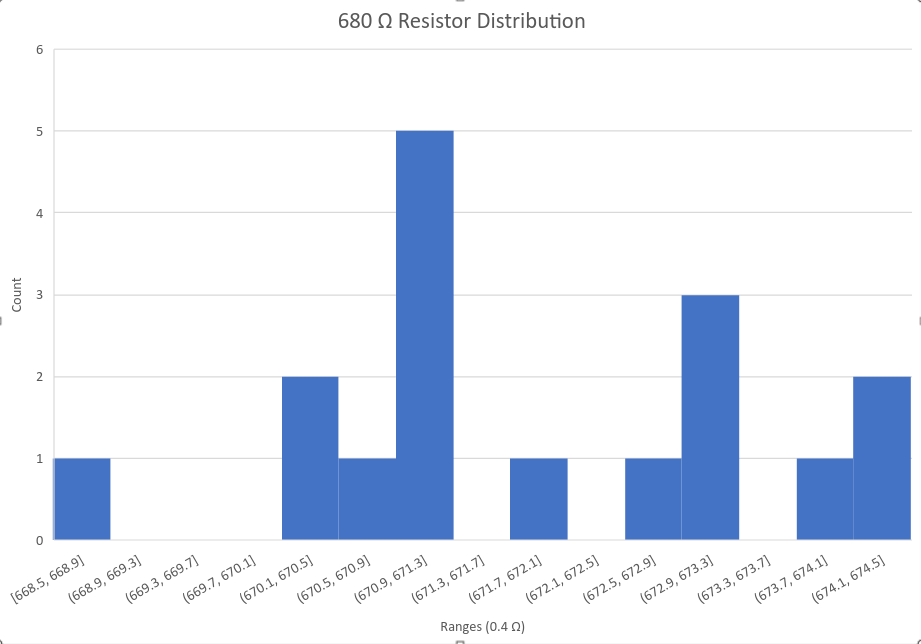
\includegraphics[width=12cm]{680_histogram}
	\end{center}
	\caption{Count vs Resistance - 680 $\Omega$ resistor histogram with 0.4 $\Omega$ bins.}
\end{figure}

\begin{figure}[H]
	\begin{center}
		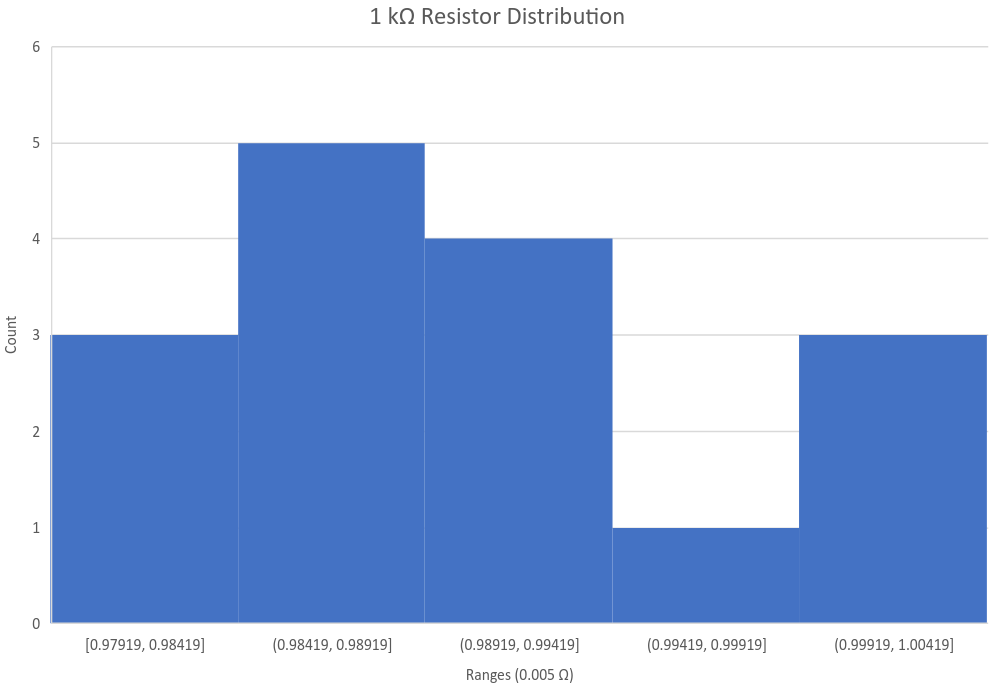
\includegraphics[width=12cm]{1k_resistor}
	\end{center}
	\caption{Count vs Resistance - 1 k$\Omega$ resistor histogram with 0.005 $\Omega$ bins.}
\end{figure}

\begin{figure}[H]
	\begin{center}
		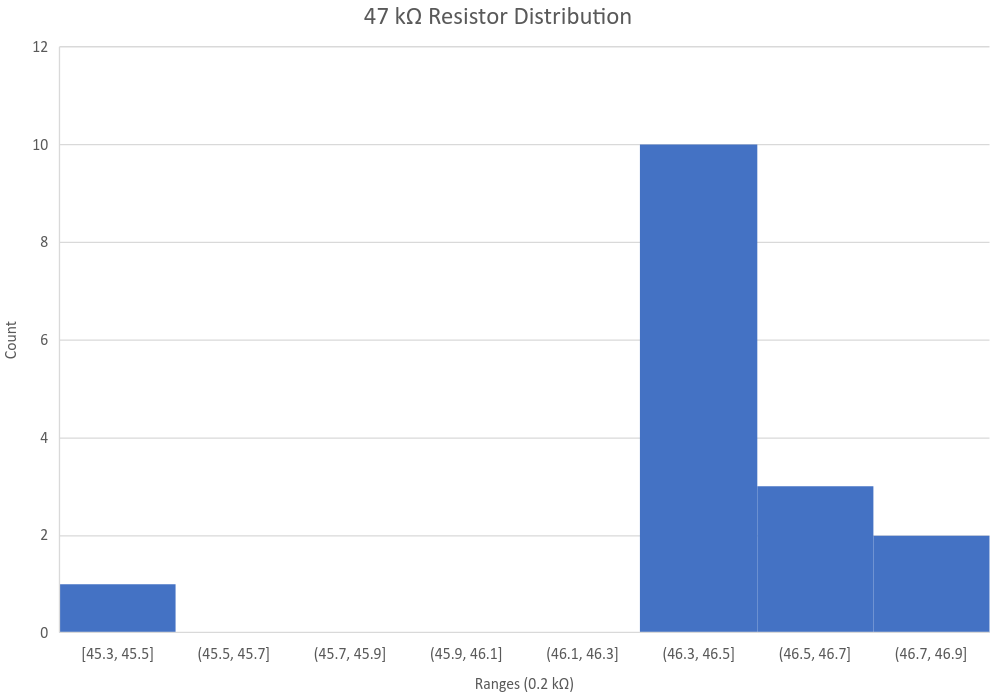
\includegraphics[width=12cm]{47k_resistor}
	\end{center}
	\caption{Count vs Resistance - 47 k$\Omega$ Resistor}
\end{figure}

\begin{figure}[H]
	\begin{center}
		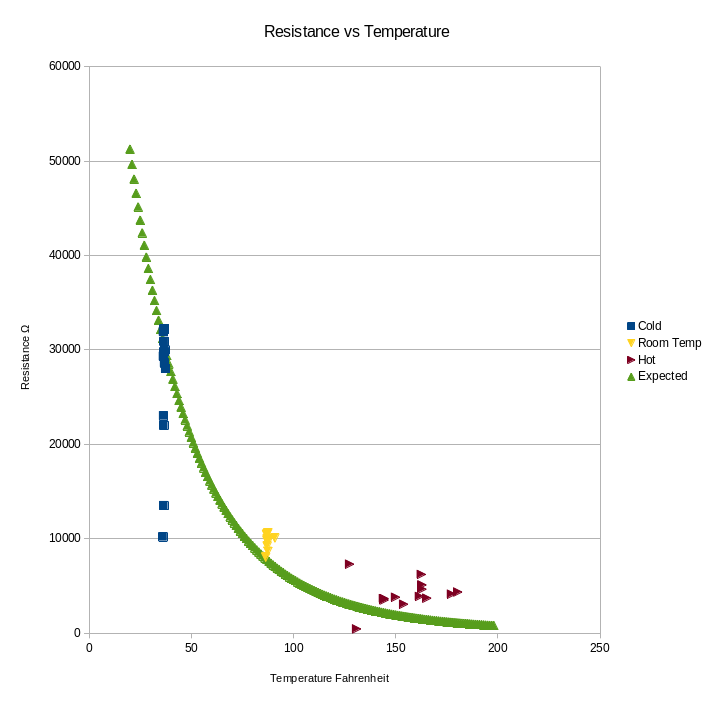
\includegraphics[width=12cm]{lab_1_thermistor_fig}
	\end{center}
	\caption{Resistance vs Temperature - Thermistor}
\end{figure}

\newpage
\section{Conclusion}
\paragraph{}
Reviewing the 680 $\Omega$ resistors reveals that one students samples had an average of 668.5 ohms. This has the largest percent difference from the nominal value. The \% difference for their samples was 1.9\%. This is still within the 5\% tolerance. From looking at the histogram (figure 3) this appears to be an outlier.
\paragraph{}
Reviewing the measurements for the 1 k$\Omega$ resistors shows us that the greatest percent difference from the nominal value is 2.08\%. The next greatest percent difference is 1.74\%. The histogram (figure 4) does not appear to indicate that this is an outlier, however I opted to use a a resolution that doesn't show as much of the spread.
\paragraph{}
Reviewing the measurements for the 47 k$\Omega$ resistors shows us that the greatest percent difference from the nominal value is 3.62\%. The value 45.3 k$\Omega$ is still within the tolerance. Referring to the histogram (figure 5) shows us that most measured values where 46.3 k$\Omega$ and 46.5 k$\Omega$.
\paragraph{}
All of the reported values for the resistor are within their tolerance.

\subsection{Thermistor Plot}
As we can see from figure 6 the resistance of the cold measurements has the widest range. This could be caused by students being impatient and not letting the thermistor cool all the way. The room temperature measurements are the most consistent. The hot temperature measurements have the largest spread of temperatures. This could be caused by the kettle turning on and off. The variation between the measured resistance and the expected resistance could be due to the students not letting the thermistor stabilize, or because the thermister might not have had as good of a contact with the kettle as the temperature probe.

\subsection{Sources of Error}
There are many possible sources of error in our measurements. Below is an incomplete list of the sources.

\begin{itemize}
	\item The Sternhart-Hart equation (equation 2) is an approximation that may not be an exact match for our thermistor.
	\item Humans may be impatient waiting for the thermistor to stabilize.
	\item The digital thermometer's probe is much smaller and less rounded than the thermistor allowing it to make better contact with the kettle allowing it to have better heat transfer.
\end{itemize}


\newpage
\section{References}
\noindent
[1] Denise Thorsen, Maher Al-Badri, INTRODUCTION TO ELECTRICAL AND COMPUTER ENGINEERING, University of Alaska Fairbanks, 2022.
\newline
\newline
\noindent
[2] NTC THERMISTOR, Jameco

\end{document}